\chapter{IPFS}

IPFS stands for InterPlanetary File System and is a peer-to-peer distributed filesystem designed to make the Web faster, safer, and more open. In contrast with standard filesystems, objects in IPFS are content-addressed, by the cryptographic hash of their contents. In the case of the standard Web, when user wants some file, he needs to know on which server is a file located and the full path to the file. In IPFS user needs only to know the hash of the requested file. He does not care about the location of the file.

\begin{figure}[H]
    \centering
    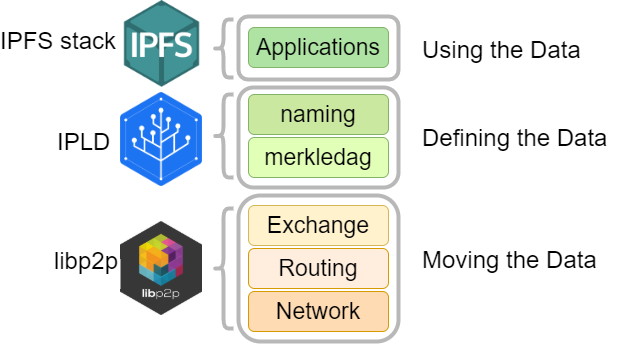
\includegraphics[width=11cm]{IPFSstack.png}
    \caption{IPFS stack}
    \label{}
\end{figure}


\subsection{Cluster}
\subsection{Node}
\subsection{CID}



\section{IPLD}
\subsection{Formats} 
\subsection{Routing} 
\subsection{Exchange} 
\subsection{Objects}  
\subsection{Files}  
\subsection{Naming (IPNM)}



